\section{\huge{Bonusopgaver}}
(til de flittige snapsedrikkere)


\subsection{Opgave 0}

Donald kan godt lide primtal, men kender kun primtallene op til 29. Hjælp ham
ved at lave en SML funktion, der finder alle primtal under 100.



\subsection{Opgave 1}
Donald skal ligesom sidste år købe julegaver til sine nærmeste venner.
Han har dog været så heldige, at de kun ønsker sig 4 forskellige slags pakker:
A, B, C og D. Donald har allerede købt gaverne, men kan ikke huske hvor meget
hver type pakke kostede. Han kan heldigvis huske hvad nogle kombinationer
af pakkerne kostede. Kan du hjælpe ham med at finde stykprisen?

\begin{align*}
A + 2B + C &= 5kr \\
2A + 3D &= 13kr \\
6B + 3C + D &= 12kr \\
A + 4C + 3D &= 12kr \\
\end{align*}

Hvor meget skal Donald betale for én af hver?

% Alle tallene bliver positive, og der er en entydig løsning. Fisse!


\subsection{Opgave 2}
Som storkunde hos internetudbyderen Donalds IP'er har du har fået tildelt
IP-adresseblokken 143.62.87.0/21. Hvor mange forskellige IP-adresser råder du
over? Angiv også den højeste og den laveste IP-adresse i dit råderum.

\subsection{Opgave 3}
Donald vil gerne lave julekort, men han vil også have, at hans computer kan
forstå hans kort. Donalds kort består heldigvis kun af ordene ``god`` og
``jul!''. Julekortene er konstrueret således, at hver gang Donald skriver
``god'' skal han også skrive ``jul!'' på et senere tidspunkt, og der skal være
lige så mange ``god'' som ``jul!''. Et eksempel på et sådant kort kunne være

\begin{center}
    god jul! god god jul! god jul! jul!
\end{center}

Kortene kan beskrives med følgende grammatik:
\begin{align*}
    G&\to J\ \$ \\
    J&\to J \text{ \ttfamily god } J \text{ \ttfamily jul! } J \\
    J&\to \varepsilon
\end{align*}
Konstruer en SLR-parsertabel over denne grammatik.


\subsection{Opgave 4}
Donald elsker IEEE standarder og har for nyligt fundet IEEE 754 til
repræsentation af tal. Hjælp ham med at omskrive tallet $173.8$ til dets
32-bit IEEE 754 repræsentation. Blev der mistet præcision?

% Svar: 01000011 00101101 11001100 11001101
% Der mistes præcision (173.800003...)

\subsection{Opgave 5}
Du skal designe en ny hjemmeside for et lille firma ved navn Donalds EDB'eri,
der sælger edb-spil til folket. Konstruer et rigt billede over situationen med
fokus på forandring. Find dernæst den mest brugervenlige farve til hjemmesiden
af følgende:
\begin{enumerate}
    \item Azurblå
    \item Marineblå
    \item Kornblomst blå
    \item Ultramarin
\end{enumerate}
Konstruer nu en papirs mock-up af hjemmesiden og foretag en fokusgruppe
undersøgelse med den relevante målgruppe. Rapporter dine resultater (ca.
60-80 sider) og giv referencer hvor nødvendigt.


\subsection{Opgave 6 - \color{red}{TODO!}}

Lav en opgave. Evt.~noget Logik eller lignende.

\subsection{Opgave 7}
Donald arbejder på en puslespilsfabrik, hvor de konstruerer en særlig slags
puslespil. Puslespillet består i at man har en masse L-formede brikker, hvor
hjørnet er sort og de to andre felter er hvide. Disse skal placeres på et
$m\times n$ bræt med hvide og sorte felter, hvor farverne skal matche. Se
eksempel på bræt og brik herunder.

\begin{figure}[htbp]
    \centering
    \vspace*{15pt}
    \begin{minipage}[h]{0.55\linewidth}
        \centering
        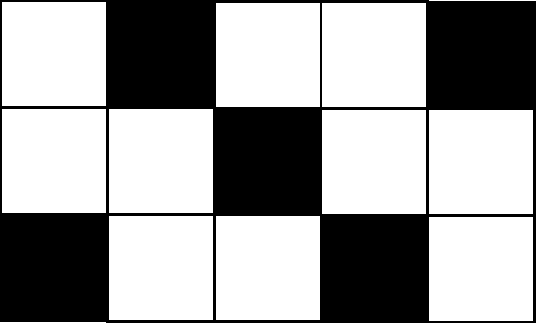
\includegraphics[width=\textwidth]{figures/braet.pdf}
    \end{minipage}
    \hspace*{.1\linewidth}
    \begin{minipage}[h]{0.2\linewidth}
        \centering
        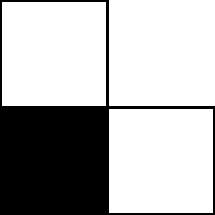
\includegraphics[width=\textwidth]{figures/brik.pdf}
    \end{minipage}
    \vspace*{15pt}
    \caption{Eksempler på et bræt (venstre) og en brik (højre) i Donalds
        puslespil. Bemærk, at brættet i dette eksempel \emph{ikke} har nogen
        løsning.}
\end{figure}

Nogle gange er det dog ikke muligt, at gå puslespillet til at gå op, så
Donald står for at checke om et givent bræt kan lade sig gøre eller ej, og
så smide brættet ud hvis det ikke kan.

Hjælp Donald, ved at lave en $O(mn)$ algoritme, der kan afgøre om et puslespil
kan gå op eller ej.

% Løses med 2SAT: Lav en variabel for om et felt er i samme brik som sin nabo for
% hver nabo. Det giver $O(mn)$ brikker. Lav nu nogle smarte conditions :P
% Kan gøres smartere ved at tælle antallet af hvide og sorte på en speciel måde.


\subsection{Opgave 8 - \color{red}{TODO!}}
Lav en opgave. Denne må gerne være fjollet eller meget svær!


\subsection{Opgave 9}

Find et tal $n$ (eller vis, at intet findes), således at følgende ligning
holder
\[
    \sum_{d|n} d = 2n + 1\ .
\]

Altså summen af $n$s divisorer $\sigma(n)$ skal være lige $2n+1$.


\textbf{\emph{NB: Der udloddes en flaske snaps til den første som kommer op i baren med en korrekt besvarelse af denne opgave!}}

% Uløstproblem. "Findes der et quasiperfekt tal?" Man ved det må være et odd
% square over 10^(35) med mindst 7 divisorer.
